\documentclass[10pt,a4paper]{article}
\usepackage[utf8]{inputenc}
\usepackage{amsmath}
\usepackage{amsfonts}
\usepackage{amssymb}
\usepackage{graphicx}
\usepackage{hyperref}
\usepackage{listings}
%\usepackage[margin=1.2in]{geometry}

\begin{document}

\def\File#1{\textsf{#1}}
\def\Code#1{\texttt{#1}}
\def\Key#1{\textsf{#1}}

\title{02220 Distributed systems}
\author{Kim Rostgaard Christensen (s084283 - \href{mailto:kroch@imm.dtu.dk}{ost})}

\maketitle

\tableofcontents

\begin{abstract}
This report describes the work done on implementing a distributed temperature monitoring network, for the course 02220 - Distributed systems using Java RMI, and apply general distributed algorithms.
\end{abstract}

\section{Introduction}
The system implemented consists of a set of inter-connected nodes that each poll a local temperature sensor at a fixed frequency. One dedicated node is appointed the role of being the master-node, or more formally the admin node. Each node (including the admin node) reports it's local sensor values back to the admin node, which then stores them.
The basic node is a system-wide root class of all nodes. All other classes inherit the functionality of this type of node.
The admin node is \emph{unique}, meaning that there can be only either 0 or 1 admin node at all times. It may suffer from temporary, or permanent failures, and therefore it must be possible to promote another node to admin. This is done via a user interface which connects to the network from an external point.

\section{The system}

For this model it was assume that the system consisted of at least four nodes - including the admin.

\subsection{Assumptions}

\begin{description}
 \item[A1] The system Contains no malicious nodes
 \item[A2] Every node has an accurate timer (not clock), so every node has the same notion of time passed, but not of absolute time
 \item[A3] A node does not change its period-count, even if disconnected.
\end{description} 
No security measures are taken in this system. The assumption is, that it is as closed loop system with no malicious nodes or individuals.\\
Processes cannot affect each other by other means than IPC. Processes can therefore not make other process stop/start/restart, or similar.

\subsection{Network topology}
Given the project description, a fitting topology would be the suggested fully-connected, divided into a fully connected network for doing reliable multicast, and a star-topology network for sending the temperature measurements to the admin node - which of course is the center of the star.

Upon system startup every node is given a unique identification that must be quantifiable - i.e. it must be comparable. For simplicity, a simple incrementing numbering scheme is chosen, starting from 0. The number of nodes and the topology is known before run-time by every node. This has to be done externally

\subsubsection{Alternate topology}
During the development of the system a number of topologies was discussed. Among these was the layered ring network, that gave some advantages when inferring causality. More details can be found in appendix \ref{sec:ring_layer_topology}.

\subsection{Choice of Java RMI}
As Java RMI (hereby also reference as merely RMI), doesn't really p
is used as a means to abstract away the socket-fiddling, and to ensure at-most-once semantics. In practice, the implementation introduces a single point of failure in having to have a central registry for all services. A remedial action for this could be to distribute the registry to several servers.
% Why not CORBA / RMI-IIOP?

\subsection{Network model}
The simulator contains an emulated network model to make monitoring easier. Every Node, including the admin, uses only RMI for communication primitives in order to enable nodes to run on different machines.

\begin{figure}[h]
\centering
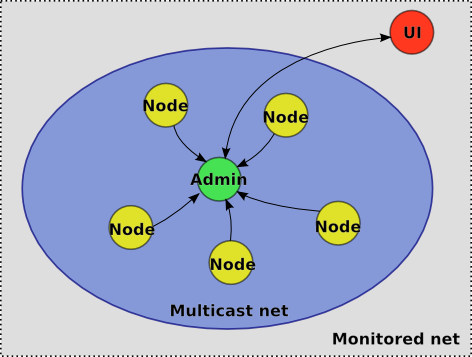
\includegraphics[scale=0.65]{fig/Networkmodel.png}
 \caption{Network model}
 \label{fig:network_model}
\end{figure}

The network model seen in figure \ref{fig:network_model} is 


Every RMI call interface is explicitly specified in the code. This gives us a safety that \emph{only} explicitly outlined calls are used throughout the system. e.g. it would be a logical contradiction to multicast a temperature message, as these always have a destination.

\subsection{Group communication}
Every node is part of a system-global multicast network that can do reliable multicast, essentially meaning that every node is fully connected. This is not depicted as edges in figure \ref{fig:network_model}, but as an ellipsis.
%TODO Alternative approaches would be to have every node maintain a list of active nodes
\section{Protocol design}
\label{sec:protocol_design}
%synchronization primitives with multicast.
\begin{description}
  \item[\Code{ID}:] Returns the Process ID of the remote reference as an integer.
  \item[\Code{latestAverage}:] Returns the latest average of measurements as a double-precision floating point value. This call is delegated to the current admin, if called on a regular node. The delegation is protected from infinite recursions.
  \item[\Code{sendMeasurement(TemperatureMessage)}:] Synchonously sends a temperature object embedded in a TemperatureMessage to a node. If the node is not an admin, it will reroute the message to the admin. Returns the a copy of the receivers VectorClock as a receipt.
  \item[\Code{send(ProposedAdminMessage)}:] Synchronously send a proposal for a new admin to a node. This receiver then returns the a copy of its VectorClock as a receipt. This follows the semantics of R-Multicast described in \cite{DistSystems}.
  \item[\Code{basicDeliver(ProposedAdminMessage)}:] Second part of the algorithm from \Code{send}. Resends all messages not previously re-sent. Returns the a copy of the receivers VectorClock as a receipt.
  \item[\Code{initialize}:] Initialize the node's internal state. Only used \emph{once} in the lifetime of a node.
  \item[\Code{startTasks}:] Start the periodic tasks of a node (see section \ref{sec:internal_tasks}). Only used \emph{once} in the lifetime of a node.
  \item[\Code{promote}:] Promotes an node to an admin (see section \ref{sec:admin_promotion}).
  \item[\Code{connectRegistry(HostString)}:] Connects the node to an RMI registry at the host supplied as argument.
  \item[\Code{disconnectRegistry}:] Disconnects a node from it's RMI registry.
\end{description} 

Each temperature object sent to the admin contains the count of the period in which it was collected.

As each admin-function related message is delegated, it removes the need for having admin-specific calls.

Furthermore there is a protocol for the network observation service, which can be seen in the file \File{ObservationServiceInterface.java}.


\subsection{Vector clocks}
Every node maintains a local vector clock that increments whenever the node changes state. This means whenever a new measurement is added, or whenever the node sends a message, the state is incremented. Whenever a node sends a message, it piggybacks its own vector clock along with the message for the receiver to merge. The receiver, upon reception of a message, sends back a receipt message containing its vector clock for the caller to merge.

- No optimizations have been done to reduce the size of vector clock messages.

\section{Regular nodes}
Nodes are RMI \Code{UnicastRemoteObject}'s classes implementing the \Code{Remote} interface.
Every node starts their life idle, and needs to be started manually using the \Code{Start()} call. For development and demonstration purposes, a bootstrapper has been developed to take care of the process launching. The bootstrapper also maintains the RMI registry, which otherwise would have to be run as separate command (\File{rmiregistry}).
Once the nodes have been started, they will register themselves as processes with their ID in the RMI registry.

\subsection{Internal tasks}
\label{sec:internal_tasks}
Each Node has two periodic tasks which together comprise a classic producer-consumer design.
\begin{description}
  \item[Transmitter:] This task is designated to emptying the transmit buffer, which is filled by the temperature sensor task. It has only this one purpose; gather messages in a circular queue and dispatch them in order. It was meant to also be able to handle re-ordering of packages to comply with either FIFO, Causal or total ordering. This feature was dropped due to increasing complexity, and lack of resources.
  \item[Temperature sensor:] This task polls it's local sensor for a value when invoked and places it, indirectly via the node, in the transmit buffer of the transmitter.
\end{description}
Both tasks are triggered by the assumed reliable timer, and thus will be have a harmonic period across all nodes.

\subsection{Promoting to admin}
\label{sec:admin_promotion}
The problem with selecting a new admin has gone through several iterations, which are described here.
\subsubsection{Mutual exclusion}
During the development phase, it was considered that using mutual exclusion could be used to assert that all nodes agreed upon the same admin, at all times. This, however, would lead to very high (and inefficient) bandwidth consumption, due to the number of messages needed to be passed around every time a node needed to send a message to the admin. It would, on the other hand, introduce total order of measurements as a side-benefit as the admin could now act as a sequencer.

\subsubsection{Agreement}
As development progressed it became apparent that the problem could be solved by the same means Byzantine generals solution, providing resilience to faulty nodes. It would follow that;
\begin{enumerate}
\item The node proposed for the new admin node is the commander.
\item Every other node are the lieutenants.
\item Every lieutenants node becomes a new (local) commander and sends each value received, to each other process (apart from the original commander) for $m$ rounds, where $m$ is the tolerated amount of failed processes.
\end{enumerate}
This system however, uses a modified (simplified) recursive version of the, more elaborately described above, OM algorithm from \cite{lamport1982byzantine}. Instead of keep initiating sending rounds, which will require all nodes to have a timeout mechanism for each round, each node resends every message with voting round increased by one - until voting round = $m-1$. As all calls are synchronous, we will eventually terminate. We would still need to keep track on who had already sent answers, though.\\\\
This algorithm was experimented with for quite some time before being abandoned. This was primarily due lack of success with getting both the fuzzy recursive OM, and the published OM implemented correctly. Secondly, it was also due to the lack of scalability due to the sheer amount of messages required to reach consensus.

\subsubsection{Reliable multicast}
\label{sec:agreement_r_multicast}
The solution selected can therefore be seen as a heuristic on both project-time remaining, messages sent and holistic system view.\\
When looking upon the system as a whole, the problem of selecting a new admin and reaching an agreement can be seen as a simple reliable broadcast - with a safety net.\\
Resilience then is provide through the routing mechanism built into the nodes, meaning that even if a node is faulty and sends a temperature message to a non-admin node, the receiving node will simply reroute the message. If a node is faulty, and claims to be the admin - all other nodes will still have the right admin. This effectively disconnects the faulty node from the network, as it will only send message to itself and can be unsubscribed from the process group using a global timeout (no measurements received) mechanism.

\section{Admin node}
The admin need to provide temperature averages to the user interface. This is done via the \Code{latestAverage} RMI interface specified in section \ref{sec:protocol_design}.
\subsection{Average temperature}
The average temperature for the user interface is calculated on the basis of the latest measurements the admin has received - from all nodes\\
To provide a consistent snapshot of the average, \textbf{A2} and \textbf{A3} was applied. This enables us to extract the temperature of each node which has the same common period, and use this for calculating an average.

\section{User interface}
The user interface is a very rudimentary and classic Java SWING interface using the JUNG framework to visualize the nodes and their connections in the network. It also visualizes the current average temperature in the system, and takes in user requests for selecting a new admin\\
The network panel uses the ``SpringLayout'' for the graph to accurately display changes to the network. This, unfortunately, has visual glitches and makes the network look a bit ``wobbly''.

\begin{figure}[h]
\centering
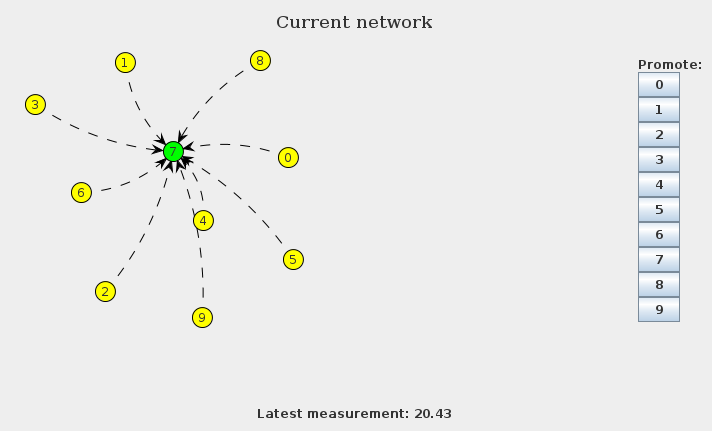
\includegraphics[scale=0.4]{fig/UI.png}
 \caption{User interface. The middle panel is the current network. The right panel has controls for promoting a new admin, and the bottom panel displays the last average temperature of the system.}
 \label{fig:ui}
\end{figure}


\section{Discussion}

\subsection{Node realization}
Every node is currently implemented as threads in the simulation of the system. They are, however, totally isolated and uses no shared memory and would be straight-forward to implement as processes. In doing this, we could give the parameters now supplied by the bootstrapper via the command line instead, or give each process a local configuration file.

\subsection{On using RMI}
A RMI interface for looking up the current list of active nodes is provide for easy availability of information. In production this would introduce a single point of failure, and make the system too vulnerable to failures.\\\\
Working with RMI has been a learning experience, but a positive one at that. It is extremely convenient to do distributed programming without having to deal with the many pitfalls of sockets, selectors, streams and file descriptors. Being able to design the protocol pseudo-formally in the Java language takes a lot of the load of having to solve general problems regarding transfers, generally.

\subsection{Replication}
\label{sec:discussion:replication}
The conceptual model of the originally designed system (see appendix \ref{sec:ring_layer_topology}) gave good opportunities for implementing replication. If the overall model of the system was reconsidered a bit, the measurements could be kept at the nodes as long as no-one wanted any averages - i.e. no user interface was subscribing to the averages. Even so, if the measurement data (within a given window) was replicated over several nodes, measurements would not need to be stored centrally, but could be located within the distributed system and fetched on-demand.\\
It would also provide opportunety to implement more sophisticated agreement algorithms, such as described in \cite{Liris-5968} and \cite{clement2009making}.

\section{Conclusion}
Reliability in distributed systems is expensive, i.e. it takes a lot communication to assert that a given state, or agreement has been reached. Therefore heuristics has been applied where they could without jeopardizing the integrity of the system. The hands-on approach to algorithms, however, is a very good way to understand them.\\
When faced with a concrete problem, it becomes easier to recollect the general solutions from the mind, and apply them specifically.\\\\
In all, the system works as intended. Alas, not with all the features originally intended. Especially the replication covered in section \ref{sec:discussion:replication} would have given some good opportunities to implement more advanced agreement algorithms.

\newpage
\appendix

\section{The ring-layer topology}
\label{sec:ring_layer_topology}
The basic idea was that every node only knew of its next-hop and it was up to the routing to decide where the message should go next. Each node would then also be a router, and every third would bridge ring networks. When having a neighbour, replication would also give some interesting opportunities to provide high-availability through redundancy. An early conceptual diagram can be seen in figure \ref{fig:old_network_model}.
This concept was abandoned eventually due to estimated implementation complexity of the shifting mechanisms. The routing mechanism is implemented, though.

\begin{figure}[h]
\centering
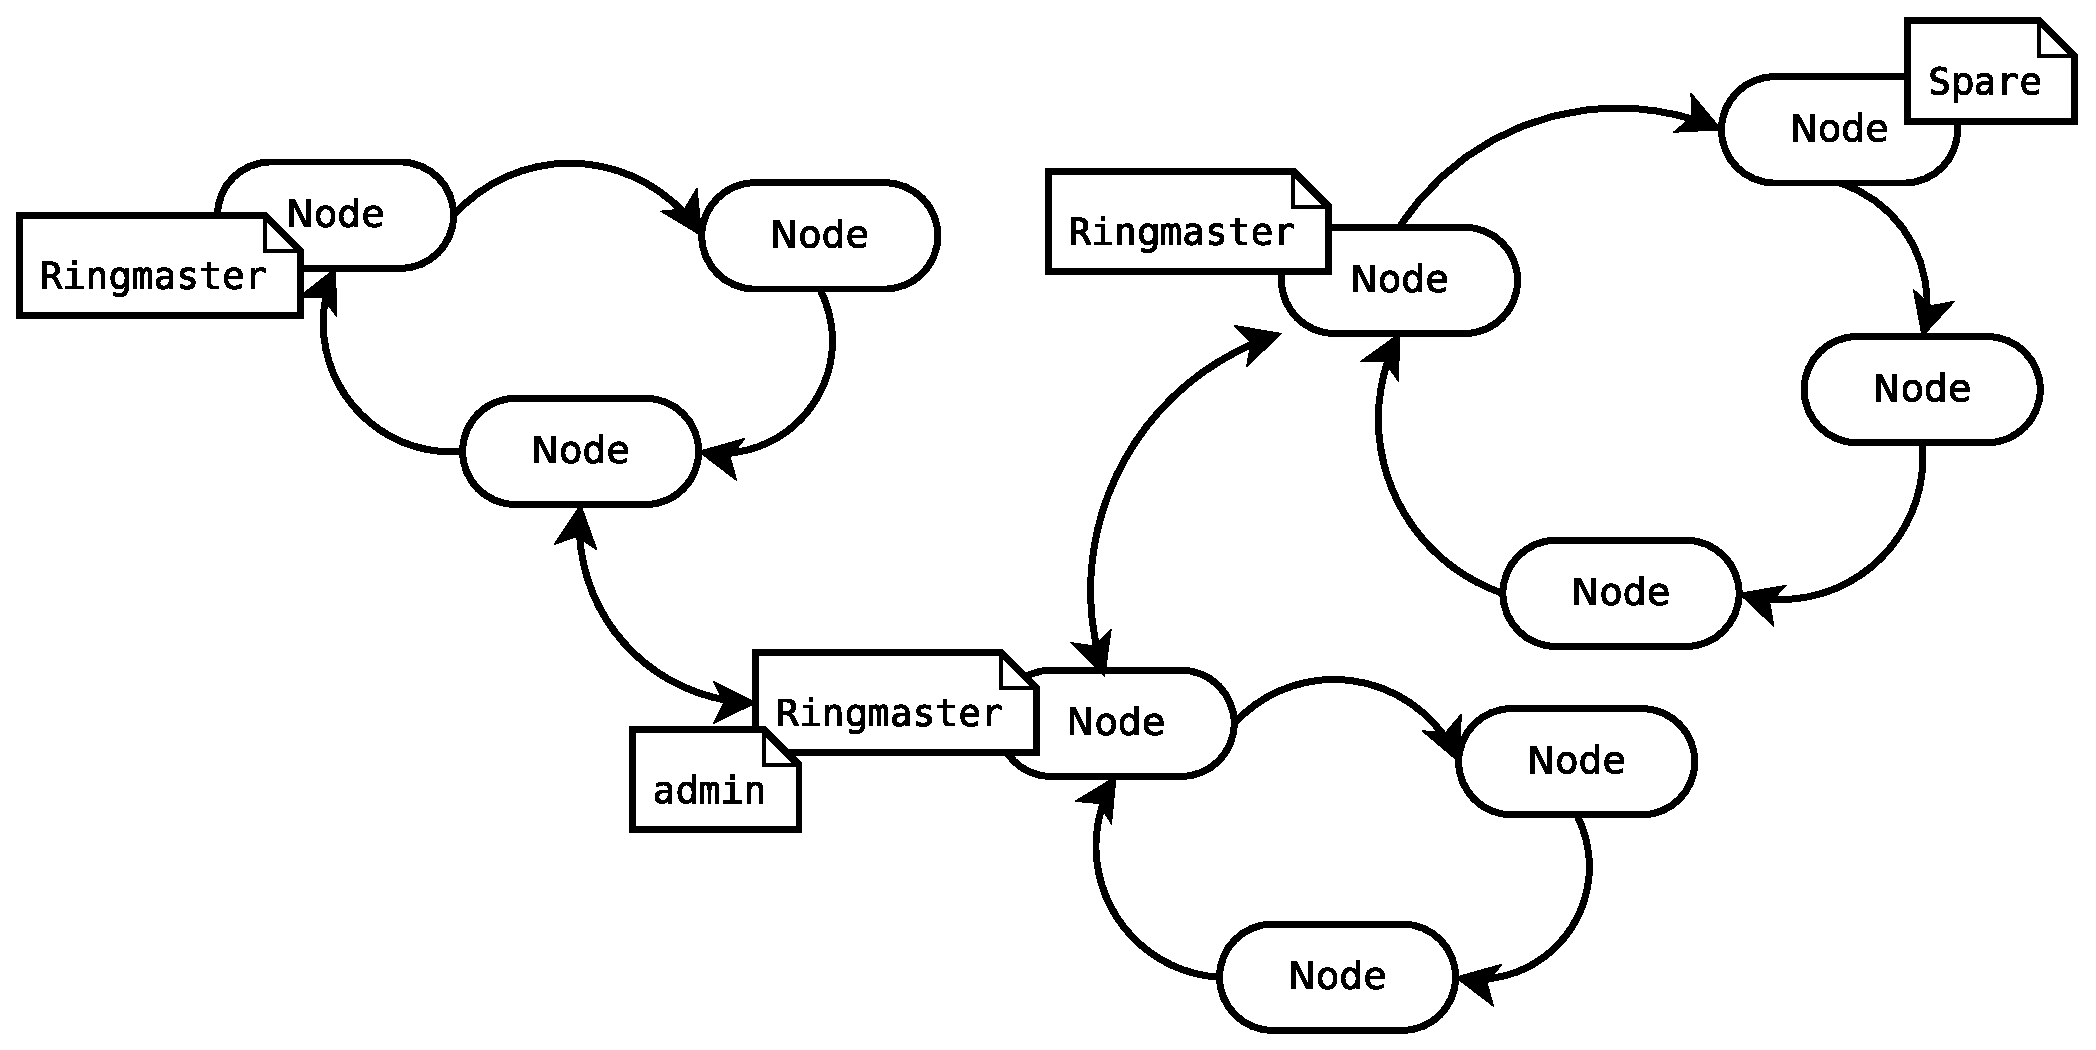
\includegraphics[scale=0.3]{fig/old_topology.eps}
 \caption{Alternate network model}
 \label{fig:old_network_model}
\end{figure}

\bibliographystyle{plain}
\bibliography{references}  % sigpr

\nocite{DistSystems}

\end{document}
